\documentclass[11pt,pdf,hyperref={unicode}]{beamer}
\usepackage[T2A]{fontenc}
\usepackage[utf8]{inputenc}
\usepackage[russian]{babel}
\usepackage{amssymb,amsfonts,amsmath,mathtext}
\usepackage{cite,enumerate,float,indentfirst}
\usepackage{graphicx}

\usetheme{Madrid}
\useoutertheme{infolines}
\usecolortheme{wolverine}
\setbeamertemplate{headline}{} % removes the headline that infolines inserts

\usepackage{amsthm}
\newtheorem{mytheorem}{Утверждение}
\theoremstyle{definition}
\newtheorem{mydefinition}{Определение}

\newcounter{saveenumi}
\newcommand{\seti}{\setcounter{saveenumi}{\value{enumi}}}
\newcommand{\conti}{\setcounter{enumi}{\value{saveenumi}}}

\DeclareMathOperator{\Tr}{Tr}

\usepackage{subfig}
\usepackage{graphicx}
\graphicspath{ {./imgs/} }


\title[]{Оптимизация статистических параметров для неравенства Эберхарда}
\author{Титова Полина, ВМ-20ш}
\date{МИЭТ, 2014г.}

\begin{document}

\begin{frame}
\titlepage
\end{frame}


\begin{frame}
\frametitle{Предпосылки рассматриваемой проблемы}
\begin{itemize}
\item Альтернатива теории о полноте квантовой механики - теория скрытых параметров, классическая вероятностная модель. Неравенства типа Бэлла хорошо подходят для проверки возможности этой теории;
\item В модели Эберхарда учитываются эффективности детекторов и возможные ложные срабатывания;
\item Для экспериментальной проверки необходимы параметры, при которых неравенство нарушается, для их подбора эффективней использовать оптимизацию.
\end{itemize}
\end{frame}

\begin{frame}
\frametitle{Цели работы}
\begin{itemize}
\item Оптимизация параметров неравенства Эберхарда таким образом, чтобы наблюдалось наиболее сильное его нарушение;
\item Нахождение параметров для случая различающихся эффективностей детекторов;
\item Использование целевой функции, учитывающей величины стандартного отклонения и исследование влияния погрешностей при установке значений параметров.
\end{itemize}
\end{frame}

\begin{frame}
\frametitle{Некоторые постулаты квантовой механики}
\begin{enumerate}
\only<1>{
  \item<1> Квантовое состояние $\psi$ - вектор комплексного гильбертового пространства, $\langle\psi, \psi\rangle = 1$.
  \item<1> Физическая наблюдаемая представляется самосопряженным оператором $A$ в гильбертовом пространстве $H$. Множество ее значений совпадает со спектром $A$.
  \item<1> В случае дискретного спектра вероятность получить собственное значение $a_m$: $P(a = a_m) = \| \pi_m^A\psi\|^2$.
  \seti
}
  \conti
  \item<2> Если в результате измерения было получено значение $a_m$, то система оказывается в состоянии $\psi_m$:
  \[
  \psi_m = \frac{\pi_m^A\psi}{ \| \pi_m^A\psi\|},
  \] 
  где $\pi_m^A: H\to H_m $ -оператор проектирования на собственное подпространство, соответсвующее $a_m$.
  \item<2> Пространство состояний объединенной системы описывается тензорным произведением $H_1 \otimes H_2$.  
\end{enumerate}
\end{frame}

\begin{frame}
\frametitle{Основы квантовой теории вероятностей}
\only<1>{
\begin{block}{Оператор плотности}
\[
\rho = \sum_ip_iP_{\psi_i},
\]
где $p_i$  - вероятность реализации состояния $\psi_i$, а $P_{\psi_i}$ - ортогональный проектор: $P_\psi: P_\psi\varphi = \langle \psi, \varphi \rangle \psi$.
\end{block}
%\begin{block}{Квантовая вероятность}
%Вероятность получить $a_i$ после измерения:
%\[
%P(A = a_i) = \Tr \rho |f_i\rangle \langle f_i|.
%\]
%где $a_i$ - собственное значение, $f_i$ - соответствующий собственный вектор.
%\end{block}
%}
%\only<2>{
\begin{block}{Мат. ожидание}
\begin{center}
$
\overline{A_\rho} \equiv \langle A\rangle = \langle A\rho, \rho\rangle = \Tr\rho A,
$
где $\Tr{}$ - след матрицы.
\end{center}
\end{block}
\begin{block}{Дисперсия}
\[
\sigma^2_{A_\rho} = \overline{\left(A_\rho - \overline{A_\rho}\right)^2} = \overline{A^2_\rho} - \overline{A_\rho}^2.
\] 
\end{block}
}
\end{frame}

\begin{frame}
\frametitle{Неравенство Эберхарда}
Четыре варианта комбинаций осей двух поляризационных призм: 
$
(\alpha_1, \beta_1), (\alpha_2, \beta_1), (\alpha_1, \beta_2), (\alpha_2, \beta_2).
$
Для каждой частицы возможно три варианта детектирования: в обыкновенном луче(о), в необыкновенном луче(е) и не была задетектирована(u).
\begin{block}{Неравенсво Эберхарда}
\begin{multline*}
J_{\mathcal{B}} = n_{uo}(\alpha_2, \beta_1) + n_{eo}(\alpha_2, \beta_1) + n_{ou}(\alpha_1, \beta_2) \\
+ n_{oe}(\alpha_1, \beta_2) + n_{oo}(\alpha_2, \beta_2) - n_{oo}(\alpha_1, \beta_1) \geq 0.
\end{multline*}
\end{block}
\end{frame}

\begin{frame}
\frametitle{Неравенство Эберхарда для квантовой механики}
\only<1>{
\begin{block}{Неравенство Эберхарда с учетом ложных срабатываний}
\[
J_{\mathcal{B}} = J_{\mathcal{B}}^{\mbox{ideal}} + 2N\zeta \geq 0,
\]
где $\zeta$ - коэффициент фонового шума для одного детектора, и 
\begin{multline*}
J_{\mathcal{B}}^{\mbox{ideal}} = n_{uo}(\alpha_2, \beta_1) + n_{eo}(\alpha_2, \beta_1) + n_{ou}(\alpha_1, \beta_2) \\
+ n_{oe}(\alpha_1, \beta_2) + n_{oo}(\alpha_2, \beta_2) - n_{oo}(\alpha_1, \beta_1) = \psi^\dagger\mathcal{B}\psi
\end{multline*}
\end{block}
\begin{block}{Предсказания квантовой механики}
\begin{eqnarray*}
n_{oo}(\alpha_1, \beta_1) = N\frac{\eta_1\eta_2}{4}\psi^\dagger[I + \sigma(\alpha_1)][I + \tau(\beta_1)]\psi,\\
n_{oe}(\alpha_1, \beta_2) = N\frac{\eta_1\eta_2}{4}\psi^\dagger[I + \sigma(\alpha_1)][I - \tau(\beta_2)]\psi,\\
n_{ou}(\alpha_1, \beta_2) = N[\eta_1(1 - \eta_2)/2]\psi^\dagger[I + \sigma(\alpha_1)]\psi,\\
\end{eqnarray*} 
\end{block}
}
\only<2>{
\begin{block}{Предсказания квантовой механики}
\begin{eqnarray*}
n_{eo}(\alpha_2, \beta_1) = N\frac{\eta_1\eta_2}{4}\psi^\dagger[I - \sigma(\alpha_2)][I + \tau(\beta_1)]\psi,\\
n_{uo}(\alpha_2, \beta_1) = N[\eta_2(1 - \eta_1)/2]\psi^\dagger[I + \tau(\beta_1)]\psi,\\
n_{oo}(\alpha_2, \beta_2) = N\frac{\eta_1\eta_2}{4}\psi^\dagger[I + \sigma(\alpha_2)][I + \tau(\beta_2)]\psi,
\end{eqnarray*} 
где
\[
\sigma(\alpha) = \left|
\begin{smallmatrix}
0 & e^{2i(\alpha - \alpha_1)} & 0 & 0\\
e^{-2i(\alpha - \alpha_1)} & 0 & 0 & 0\\
0 & 0 & 0 & e^{2i(\alpha - \alpha_1)}\\
0 & 0 & e^{-2i(\alpha - \alpha_1)} & 0
\end{smallmatrix}\right|
\] 
и 
\[
\tau(\beta) = \left|
\begin{smallmatrix}
0 & 0 & e^{2i(\beta - \beta_1)} & 0\\
0 & 0 & 0 & e^{2i(\beta - \beta_1)}\\
e^{-2i(\beta - \beta_1)} & 0 & 0 & 0\\
0 & e^{-2i(\beta - \beta_1)} & 0 & 0
\end{smallmatrix}\right|
\]
\end{block}
}
\end{frame}

\begin{frame}
\frametitle{Параметры оптимизации}
Примем $\alpha_1 - \alpha_2 = \beta_1 - \beta_2 = \theta$ и $\zeta = 0$, так как он вносит константный вклад в $J/N$. 

Состояние квантовой системы будем искать в виде
\[
\psi = \frac{1}{2\sqrt{1 + r^2}}\left|
\begin{smallmatrix}
(1+r)e^{-i\omega}\\
-(1 - r)\\
-(1 - r)\\
(1 + r)e^{i\omega}
\end{smallmatrix}\right|,
\]
где $0 \leq r \leq 1$, $\alpha_1 = \omega / 2 - 90^\circ$ и $\beta_1 = \omega / 2$.
\end{frame}

\begin{frame}
\frametitle{Результаты для случая различающихся эффективностей}
\begin{figure}[h]
	\subfloat[Зависимость $\theta(\eta_1, \eta_2)$]{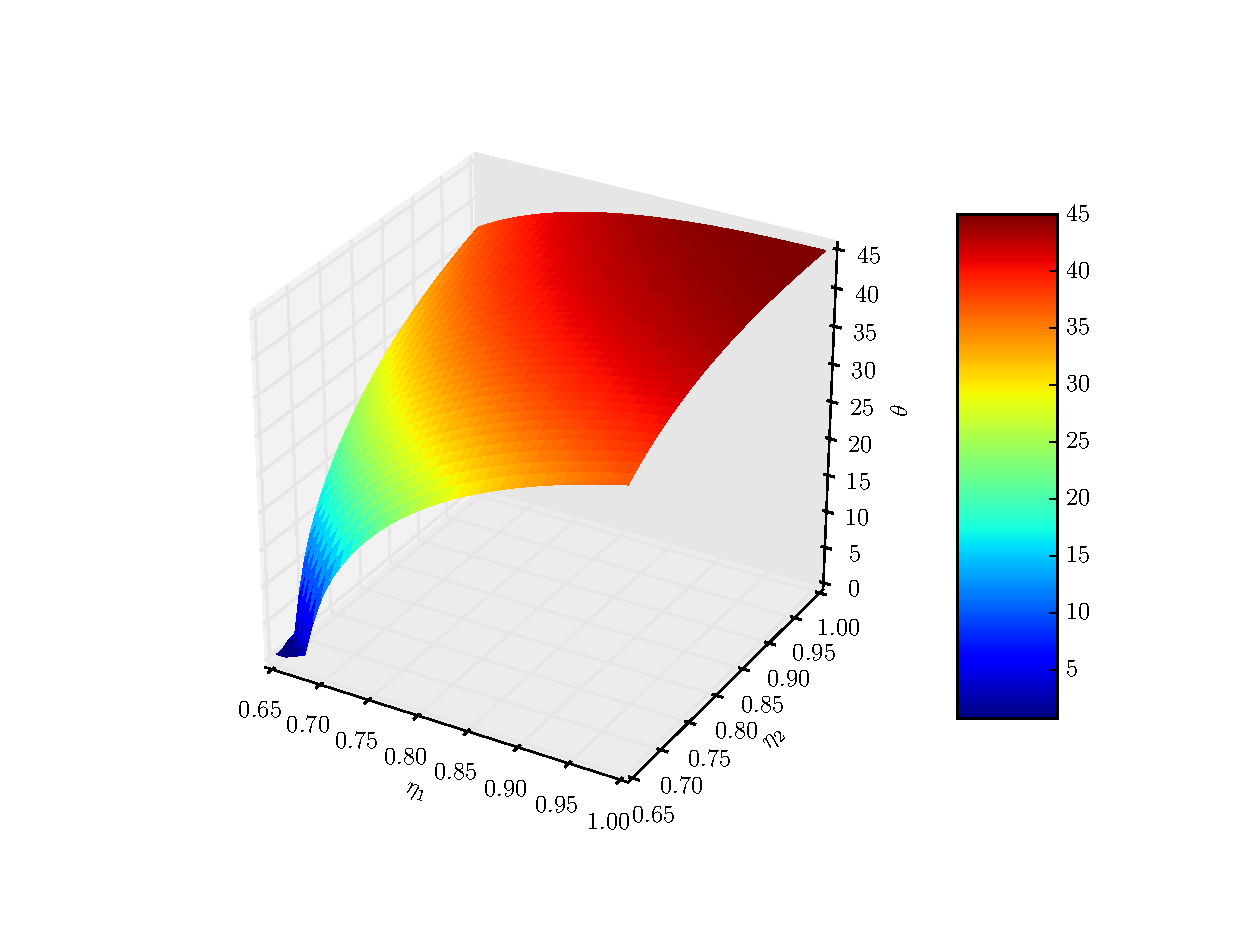
\includegraphics[width=0.5\linewidth]{theta3d.eps}}
	\subfloat[Зависимость $J(\eta_1, \eta_2) / N$]{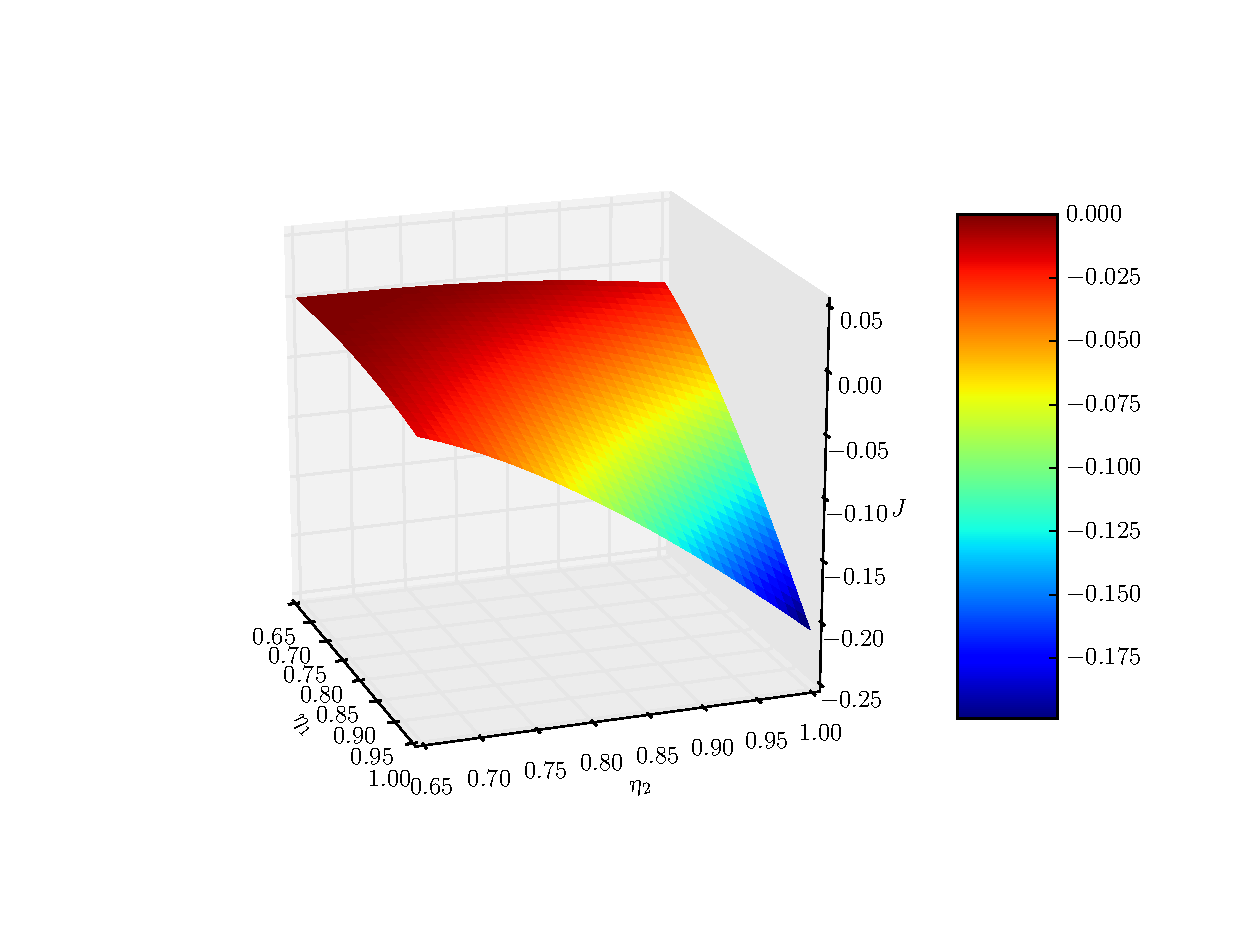
\includegraphics[width=0.5\linewidth]{J3d.eps}}
\end{figure}
\end{frame}

\begin{frame}
\frametitle{Оптимизация параметров для модели Цайлингера}
\begin{block}{Модель}
Основное отличие от модели Эберхарда - другое квантовое состояние:
\[
\rho = \frac{1}{\sqrt{1+r^2}}\left|
\begin{smallmatrix}
0 & 0 & 0 & 0\\
0 & 1 & Vr & 0\\
0 & Vr & r^2 & 0\\
0 & 0 & 0 & 0
\end{smallmatrix}\right|
\]
\end{block}

В результате оптимизации по четырем углам в отдельности получились следующие параметры:

\begin{tabular}{|c|c|c|c|c|c|}
\hline 
 & $\alpha_1$ & $\alpha_2$ & $\beta_1$ & $\beta_2$ & $J$ \\ 
\hline 
Результаты из статьи & 85.6 & 118.0 & -5.4 & 25.9 & -120191 \\ 
\hline 
Результаты оптимизации & 85.0 & 115.1 & -4.0 & 27.4 & -126060 \\ 
\hline 
\end{tabular}
\end{frame}

\begin{frame}
\frametitle{Оптимальное квантовое состоянии для целевой функции $J_\mathcal{B}$}
\begin{mytheorem}
Квантовое состояние $\psi$, минимизирующее целевую функцию $J$, является собственным вектором матрицы $\mathcal{B}$ и обращает дисперсию в ноль.
\end{mytheorem}
\begin{proof}
По теореме Куранта-Фишера $\lambda_1 \leq \langle\mathcal{B}\psi, \psi\rangle \leq \lambda_n$, где $\lambda_1, \ldots \lambda_n$ - собственные значения, отсортированные в порядке возрастания. Минимум $J_\mathcal{B} = \langle\mathcal{B}\psi, \psi\rangle = \lambda_1$ достигается при $\psi = \psi_1$ - собственный вектор. 

Для величины дисперсии в этом случае имеем:
\[\sigma^2 = \langle B^2\rangle - \langle B\rangle^2 = \psi^\dagger B^2 \psi - \lambda_1^2 = \psi^\dagger B \lambda_1  \psi - \lambda_1^2 = 0.
\]

\end{proof}
\end{frame}

\begin{frame}
\frametitle{Целевая функция с учетом величины стандартного отклонения}
\begin{block}{Целевая функция}
\[
K = \frac{J_\mathcal{B} }{\sigma}
\]
\end{block}
Рассмотрим $\theta' = \theta + \xi$, где $\xi$ - случайная величина, равномерно распределенная на отрезке $[-\delta; \delta]$, $\delta > 0$ - параметр разброса. Тогда
\[
J_\mathcal{B} = \frac{1}{2\delta}\int_{-\delta}^\delta \langle \mathcal{B}(r, \omega, \theta + x)\psi, \psi \rangle dx
\] и
\[
\sigma^2 = \frac{1}{2\delta}\int_{-\delta}^\delta (\langle \mathcal{B}^2(r, \omega, \theta + x)\psi, \psi \rangle - \langle \mathcal{B}(r, \omega, \theta + x)\psi, \psi \rangle^2) dx.
\]
\end{frame}

\begin{frame}
\frametitle{Полученные параметры}
\begin{figure}[h]
	\subfloat[Зависимость $\theta(\eta)$]{\includegraphics[width=0.5\linewidth]{theta_ang.eps}}
	\subfloat[Зависимость $J(\eta) / N$]{\includegraphics[width=0.5\linewidth]{J_ang.eps}}
\end{figure}
\end{frame}

\begin{frame}
\frametitle{Обобщение предыдущего случая на все 4 угла в отдельности}
Пусть каждый из углов $\alpha_1, \alpha_2, \beta_1, \beta_2$ задается с помощью случайной величины $\varphi' = \varphi + \xi$, где $\xi$ - случайная величина из предыдущего случая.
\begin{block}{Мат. ожидание и дисперсия}
\[
J_\mathcal{B} = \frac{1}{16\delta^4}\int\int\int\int_{-\delta}^\delta \langle \mathcal{B}(x_1, x_2, x_3, x_4)\psi, \psi \rangle dx_1dx_2dx_3dx_4,
\] 
\[
\sigma^2 = \frac{1}{16\delta^4}\int\int\int\int_{-\delta}^\delta (\langle \mathcal{B}^2\psi, \psi \rangle - \langle \mathcal{B}\psi, \psi \rangle^2) dx_1dx_2dx_3dx_4.
\]
\end{block}
\end{frame}

\begin{frame}
\frametitle{Полученные параметры}
\begin{figure}[h]
	\subfloat[Зависимость $\theta(\eta)$]{\includegraphics[width=0.5\linewidth]{theta_4ang.eps}}
	\subfloat[Зависимость $J(\eta) / N$]{\includegraphics[width=0.5\linewidth]{J_4ang.eps}}
\end{figure}
\end{frame}

\begin{frame}
\frametitle{Заключение}
\begin{itemize}
\item Были найдены оптимальные параметра неравенства Эберхарда для случая различающихся эффективностей детекторов.
\item Оптимизация параметров для параметров Цайлингера позволила получить другие значения углов, которые еще сильнее нарушают неравенство.
\item Было проведено нахождение параметров с учетом возможных погрешностей в установке углов в ходе эксперимента. Она выявила малый разброс значений целевой функции при варьировании величины погрешностей. Это позволяет предположить, что в ходе эксперимента можно ослабить контроль над точностью установки осей поляризационных призм.
\end{itemize}
\end{frame}

\end{document}